\section{Experimental Results} \label{sec:experiments}

The goal of this section is to investigate the limits of the naive sampling method which serves as benchmark for the proposed control framework. To this end, we define the following metrics:
\begin{itemize}
    \item \textit{average stage cost}: this performance metric is computed averaging the stage cost evaluated at each time step. Task duration and cost scheduling is kept fixed among all the experiments.  
    \item \textit{cumulative constraints violation}: as each barrier function is, by definition, negative outside of the safe set, we define the following metric as a proxy to the size of the constraint violation along the duration of an experiment:
    \begin{equation*}
        v^{tot}_i = \sum\limits_{t=0}^{T_{exp}} \max(0, -h_i(\vect{x}_t))
    \end{equation*}
    referring to the i\textsuperscript{th} barrier function and associated constraint.
    \item \textit{average interaction wrench}: average wrench which is exerted to the environment during the execution of the task
    \item \textit{dissipated power}: during an ideal interaction with an articulated object, power is not dissipated, meaning that the control doesn't act against the environmental constraint. We use the dissipated power as an efficiency metric:
    \begin{equation}
        P_{diss} = \sum\limits_{0}^{T_{exp}} -\command^T \boldsymbol{\tau}_{ext}
    \end{equation}
\end{itemize}
The simulation experiments are conducted on a dynamic manipulator model as described by \eqref{eq:eom}. The manipulation tasks consist in maneuvering different articulated objects. The articulated objects in the task are a \textit{shelf}, \textit{dishwasher}, \textit{microwave} and \textit{drawer} as shown in \fig\ref{fig:object_manipulation}. They differ in type and orientation of the joint. The \textit{shelf} and \textit{microwave} have a vertical revolute joint while the \textit{dishwasher} has a horizontal revolute joint. Ultimately, the \textit{drawer} has a horizontal prismatic joint. As the goal is to reproduce as close as possible the real manipulator, the simulation is run with a rate of 1000 Hz. The simulated manipulator is controlled using a PI velocity low-level controller, as its real counterpart and we model imperfect velocity tracking assuming that non-linear terms are not perfectly compensated. 
  
\begin{figure}[t]
\centering
  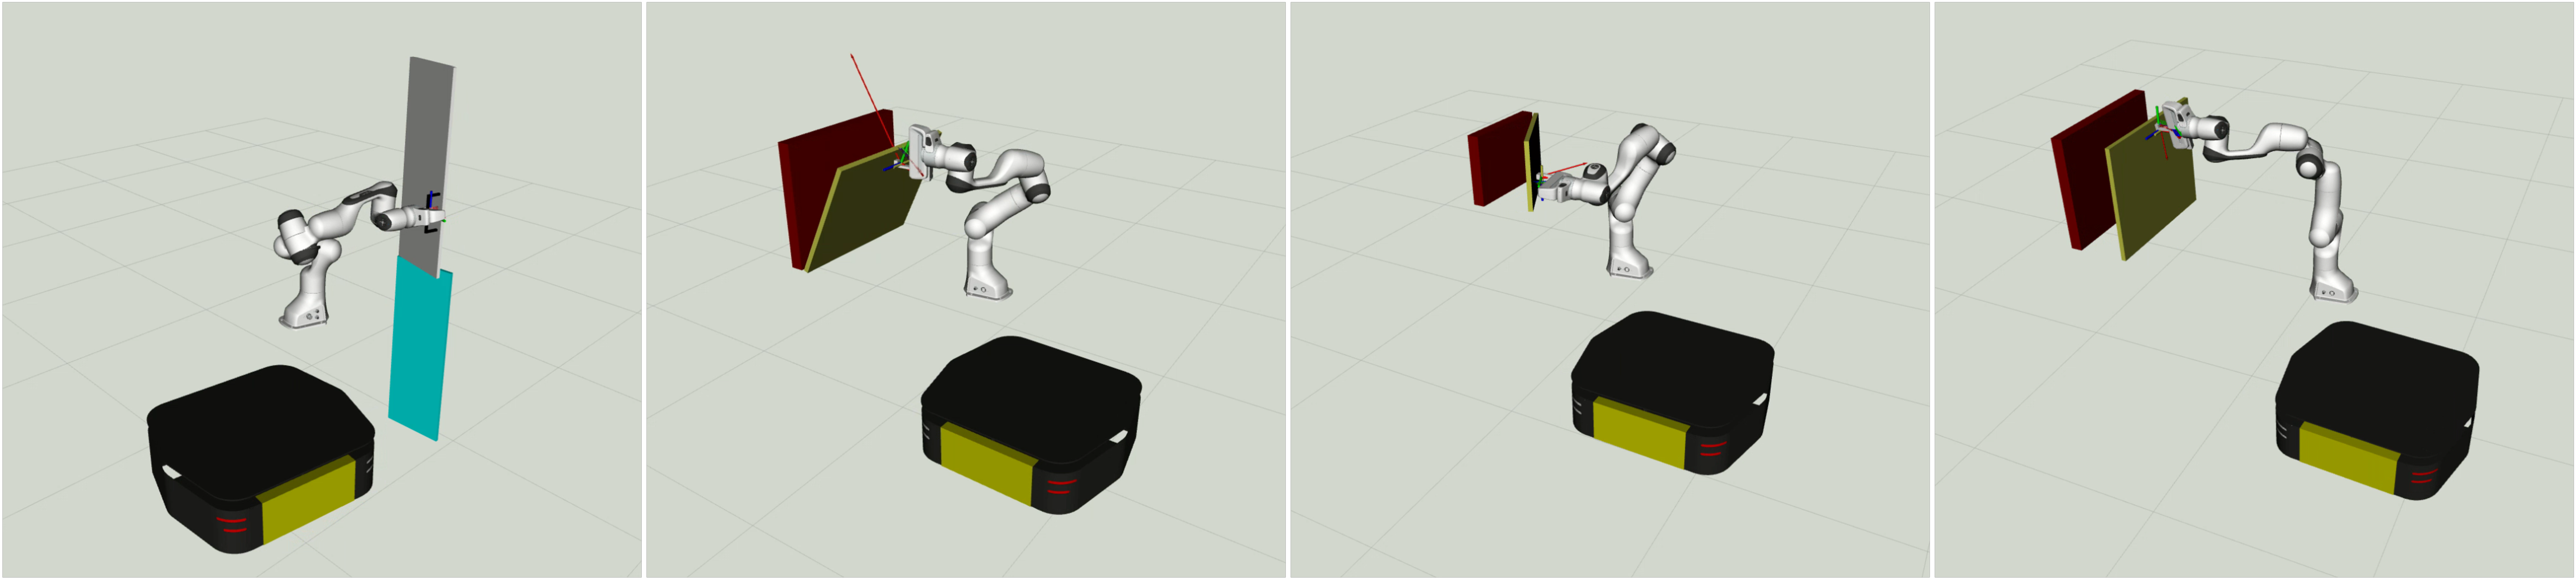
\includegraphics[width=\columnwidth]{figures/articulated_objects_sim.pdf}
  \caption{The four articulated objects used in our simulation evaluations. From left to right: shelf, dishwasher, microwave, drawer.} \label{fig:object_manipulation}
\end{figure}

\subsection{Power consumption}
In this experiment we look at the effect of the power term in the task execution. As we can see in \fig \ref{fig:power_cost_comparison}, the power cost is effective in decreasing the energy dissipation during the manipulation task. For each of the experiments where the power cost is active we set $w_p=10$ and $p_{max} = 0.0$. For all experiments we use $50$ samples as they are a good trade-off between control-frequency and performance. We observe that in all experiments the robot is able to accomplish the task (fully open the articulated object). This experiment shows that we can use wrench information to encode even more complex tasks. One for example, can think of shaping an \textit{information-theoretic} cost that seek useful wrench measurement to estimate the system model (TODO repharse or put in future works). 

\begin{figure}[t]
\centering
  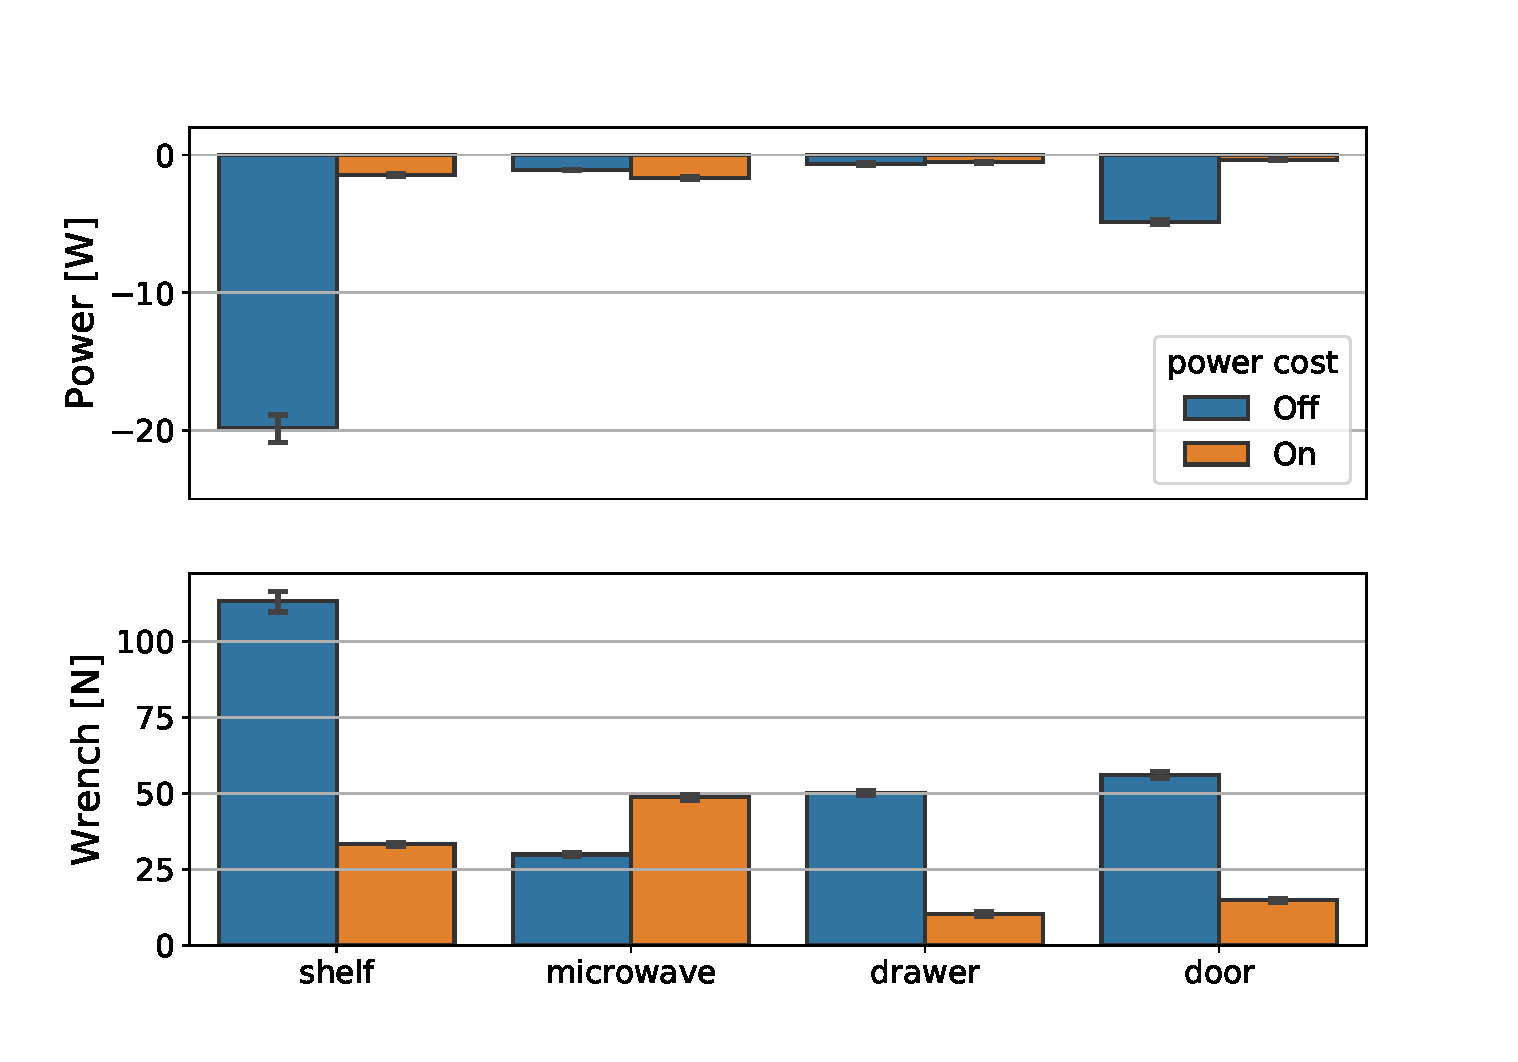
\includegraphics[width=\columnwidth]{figures/methods_comparison/power_cost.pdf}
  \caption{The first figures shows the power dissipated and wrench norm distribution for each manipulated object. As a beneficial side effect also the interaction wrench is reduced. Only for the microwave this is not the case but we see that even without this cost term, sampling is enough to find \textit{low power} trajectories.} \label{fig:power_cost_comparison}
\end{figure}


\subsection{Methods comparison}
We aim to compare the control framework in a challenging interaction scenario. In all the experiments the robot starts in configuration which is close to the arm joint limits and self collision. The base of the robot is at $(-3.0, -3.0)$ outside of the prescribed position limits of $[(2.0, 2.0), (-2.0, -2.0)]$. We perform ten experiments for each articulated object and we compare four control methods:
\begin{itemize}
    \item \textit{no\textunderscore filter}: only sampling is used to generate velocity commands,
    \item \textit{filter\textunderscore out}: the velocity command is passed at every time step of the low-level controller through the FILTER-QP,
    \item \textit{filter\textunderscore in}: the velocity trajectory is passed through the FILTER-QP before being sent to the low-level controller. This is then fed back to the sampling procedure as described in \algo \ref{algo:sequential_qp},
    \item \textit{filter\textunderscore in\textunderscore out}: a combination of the previous two methods where the FILTER-QP is used to transform velocity trajectories and at a higher rate in the low-level control loop (see \fig \ref{fig:cascaded_architecture})
\end{itemize}
The results of the experiments are summarized in \fig \ref{fig:methods_comparison}. In all cases, filtering the velocity commands has a beneficial effect. The drastic reduction of cumulative joint limits violation shows that closing the loop between the filter and the sampling allows to react more quickly to constraints violation and suggests that we are able to generate trajectories that recover from constraints violation. We can observe also a reduction of the violation of self collision and reach constraints, but in this case the improvement of  \textit{filter\textunderscore in\textunderscore out} with respect to \textit{filter\textunderscore in} is not as prominent. We hypothesize that this is due to a low likelihood of getting into self-collision given the task and robot morphology. Considering dissipated power, we see that the overall trend is a more efficient task execution. Positive values for the shelf case, show that desired velocity has the same direction as the external force, resulting in a more compliant autonomous behavior. This will become more evident in the next experiment where we simulate a model mismatch which might lead to high interaction forces. 
\begin{figure}[t]
\centering
\hspace*{-0.4cm} 
\begin{subfigure}{\columnwidth}
    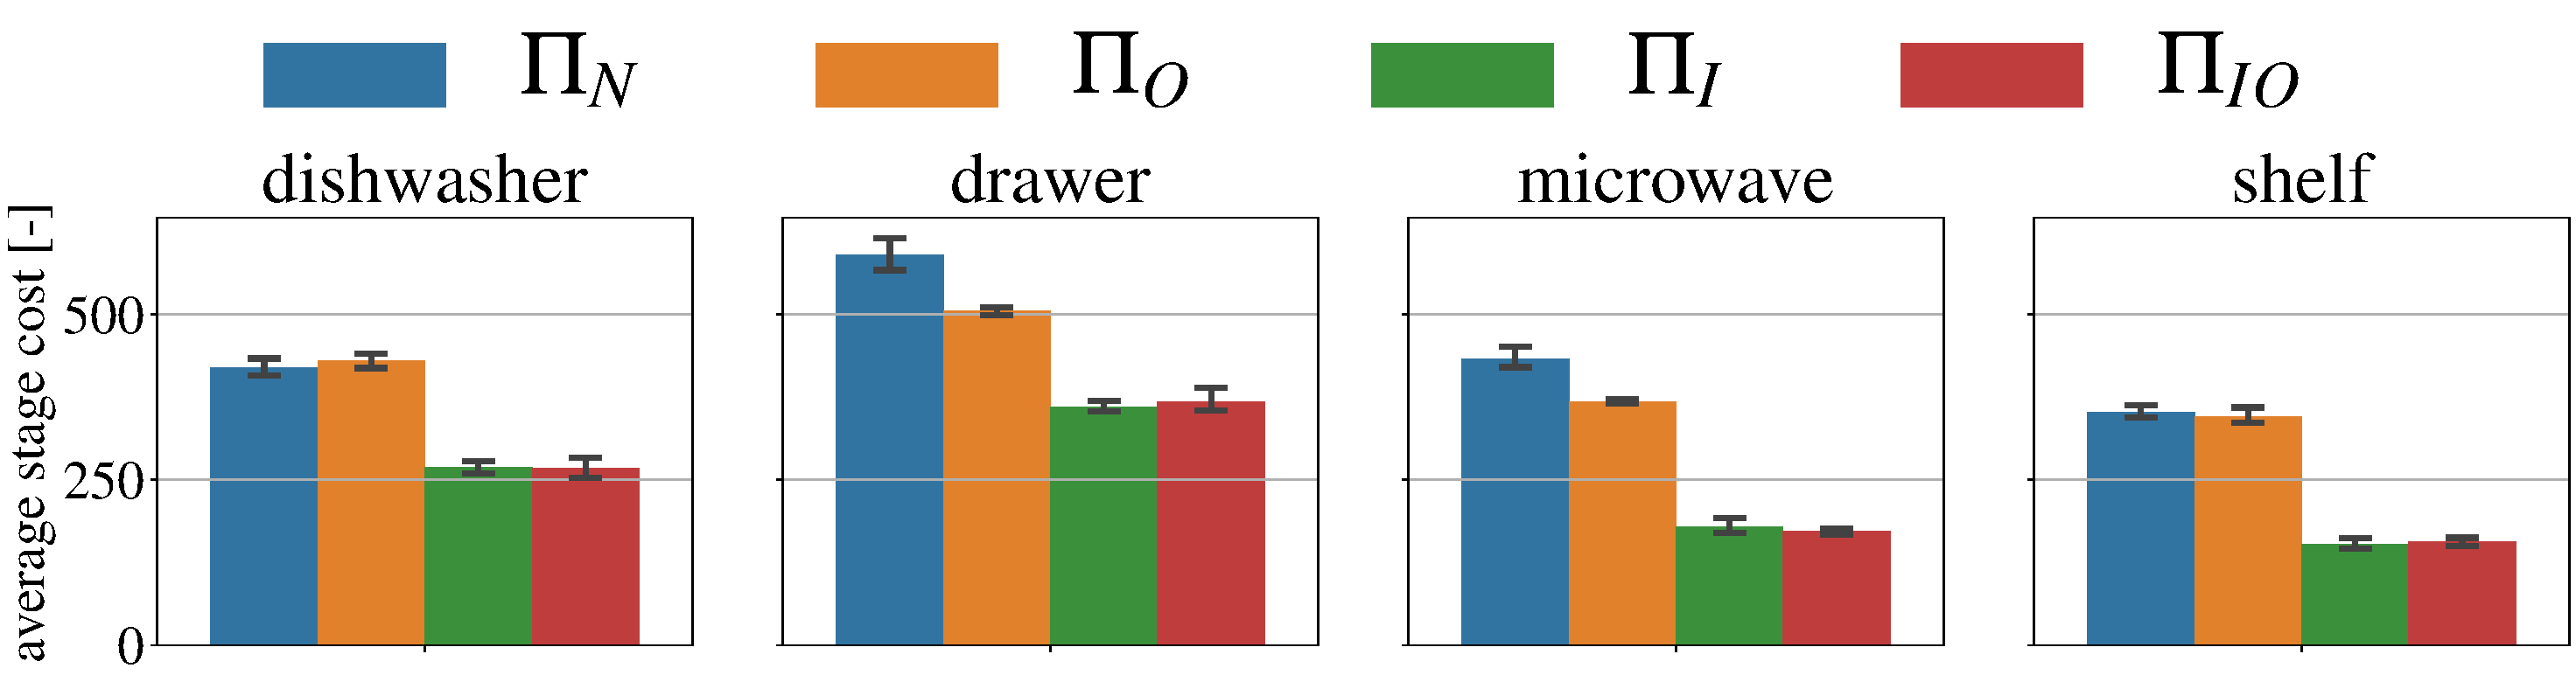
\includegraphics[width=\linewidth]{figures/methods_comparison/average_stage_cost.pdf}
\end{subfigure}%
\hfill
\hspace*{-0.4cm} 
\begin{subfigure}{\columnwidth}
    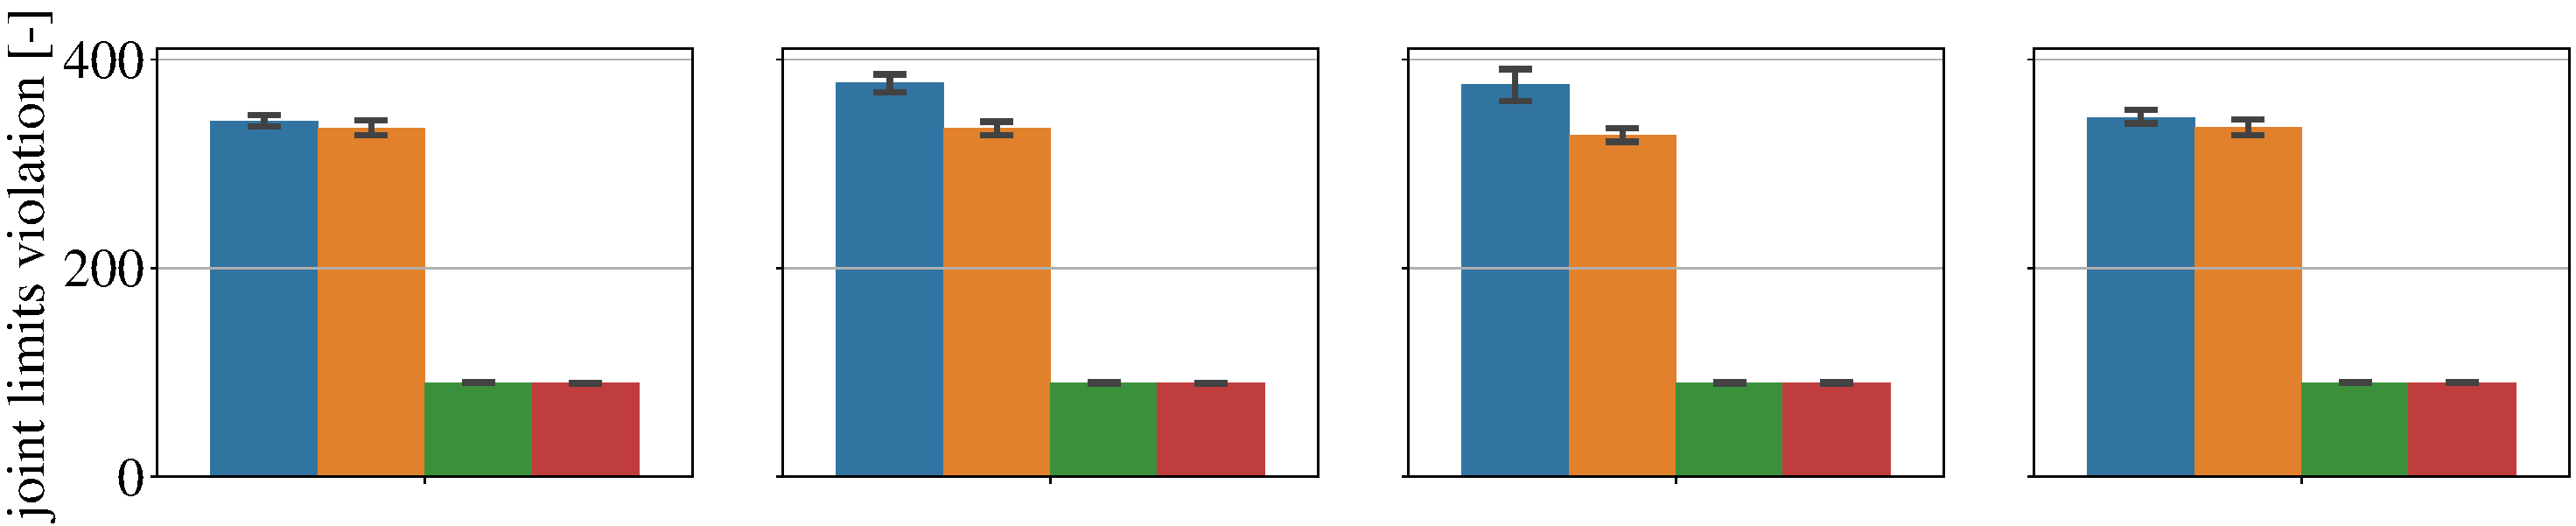
\includegraphics[width=\linewidth]{figures/methods_comparison/joint_limits.pdf}
\end{subfigure}%
\hfill
\hspace*{-0.4cm} 
\begin{subfigure}{\columnwidth}
    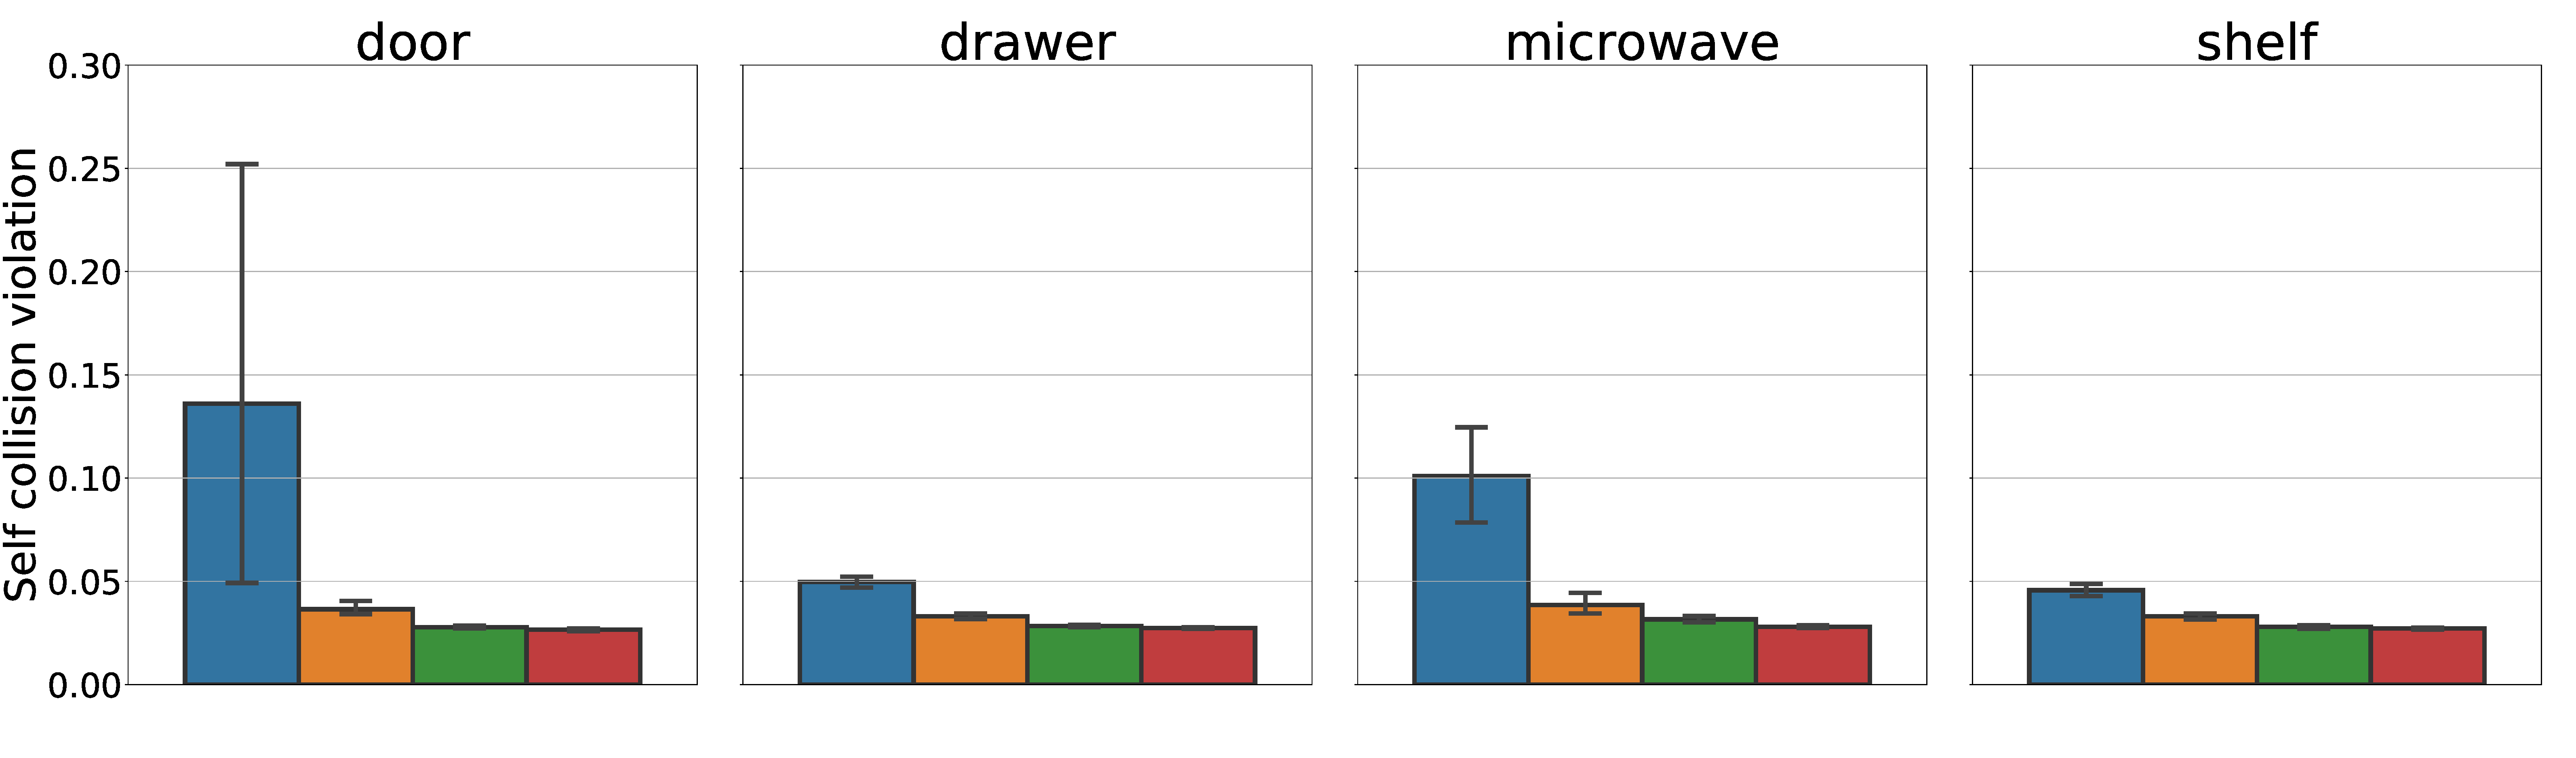
\includegraphics[width=\linewidth]{figures/methods_comparison/self_collision.pdf}
\end{subfigure}
\hspace*{-0.4cm} 
\begin{subfigure}{\columnwidth}
    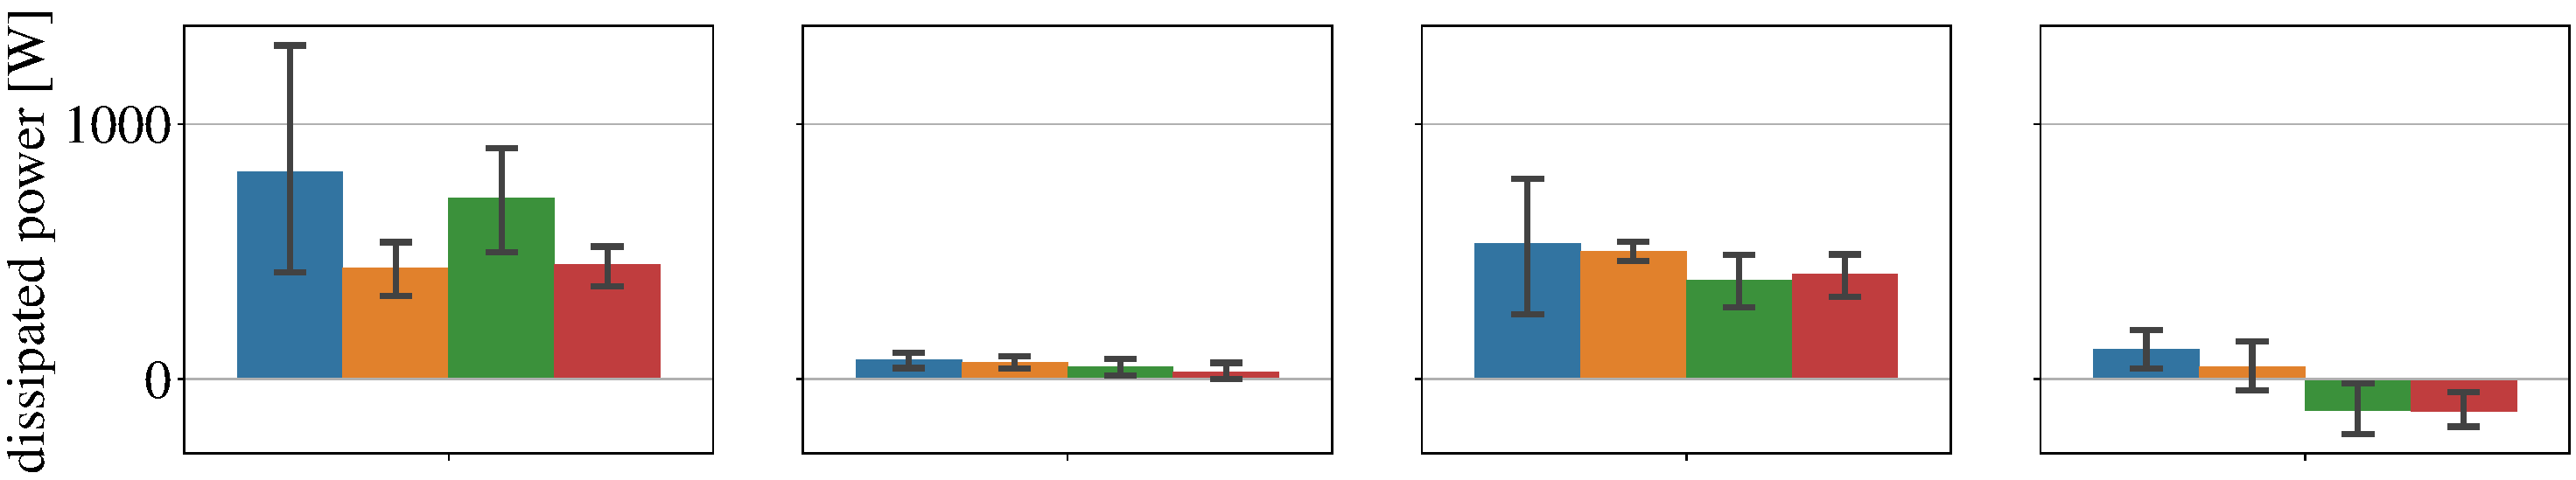
\includegraphics[width=\linewidth]{figures/methods_comparison/dissipated_power.pdf}
\end{subfigure}
\hfill
\caption{This figure shows a comparison between the different control methods when the FILTER-QP is used in different stages of the cascaded architecture. Results are separate by manipulation task. The self-collision metric accounts also for the arm-reach constraint as they share the same implementation.}\label{fig:methods_comparison}
\end{figure}

\subsection{Interaction wrench}
We want to investigate if the controller can reason about interaction wrench through the power cost described in \eqn \ref{eq:power_cost}. This is a novel algorithmic component, as it enables indirect control of the interaction wrench. 

\subsection{Robust interaction}
In this experiment we aim to show that the tank is effective in limiting the dissipated power and thus generating a stable and robust interaction behavior. We design an interaction scenario where the articulated object gets stuck during motion. In the simulated experiments we fix the object position for $5s$. After this time the object is release and free to move. We can note that when the SAFETY-QP is turned off and therefore no passivity is ensured, the negative power flow is not bounded, leading to high interaction wrenches. On the other hand, when the energy tank is used, only a maximal amount of energy, namely that stored in the tank can be used, regulating the overall interaction wrench.    

\begin{figure}[t]
\centering
\hspace*{-1.35cm} 
\begin{subfigure}{1.3\columnwidth}
    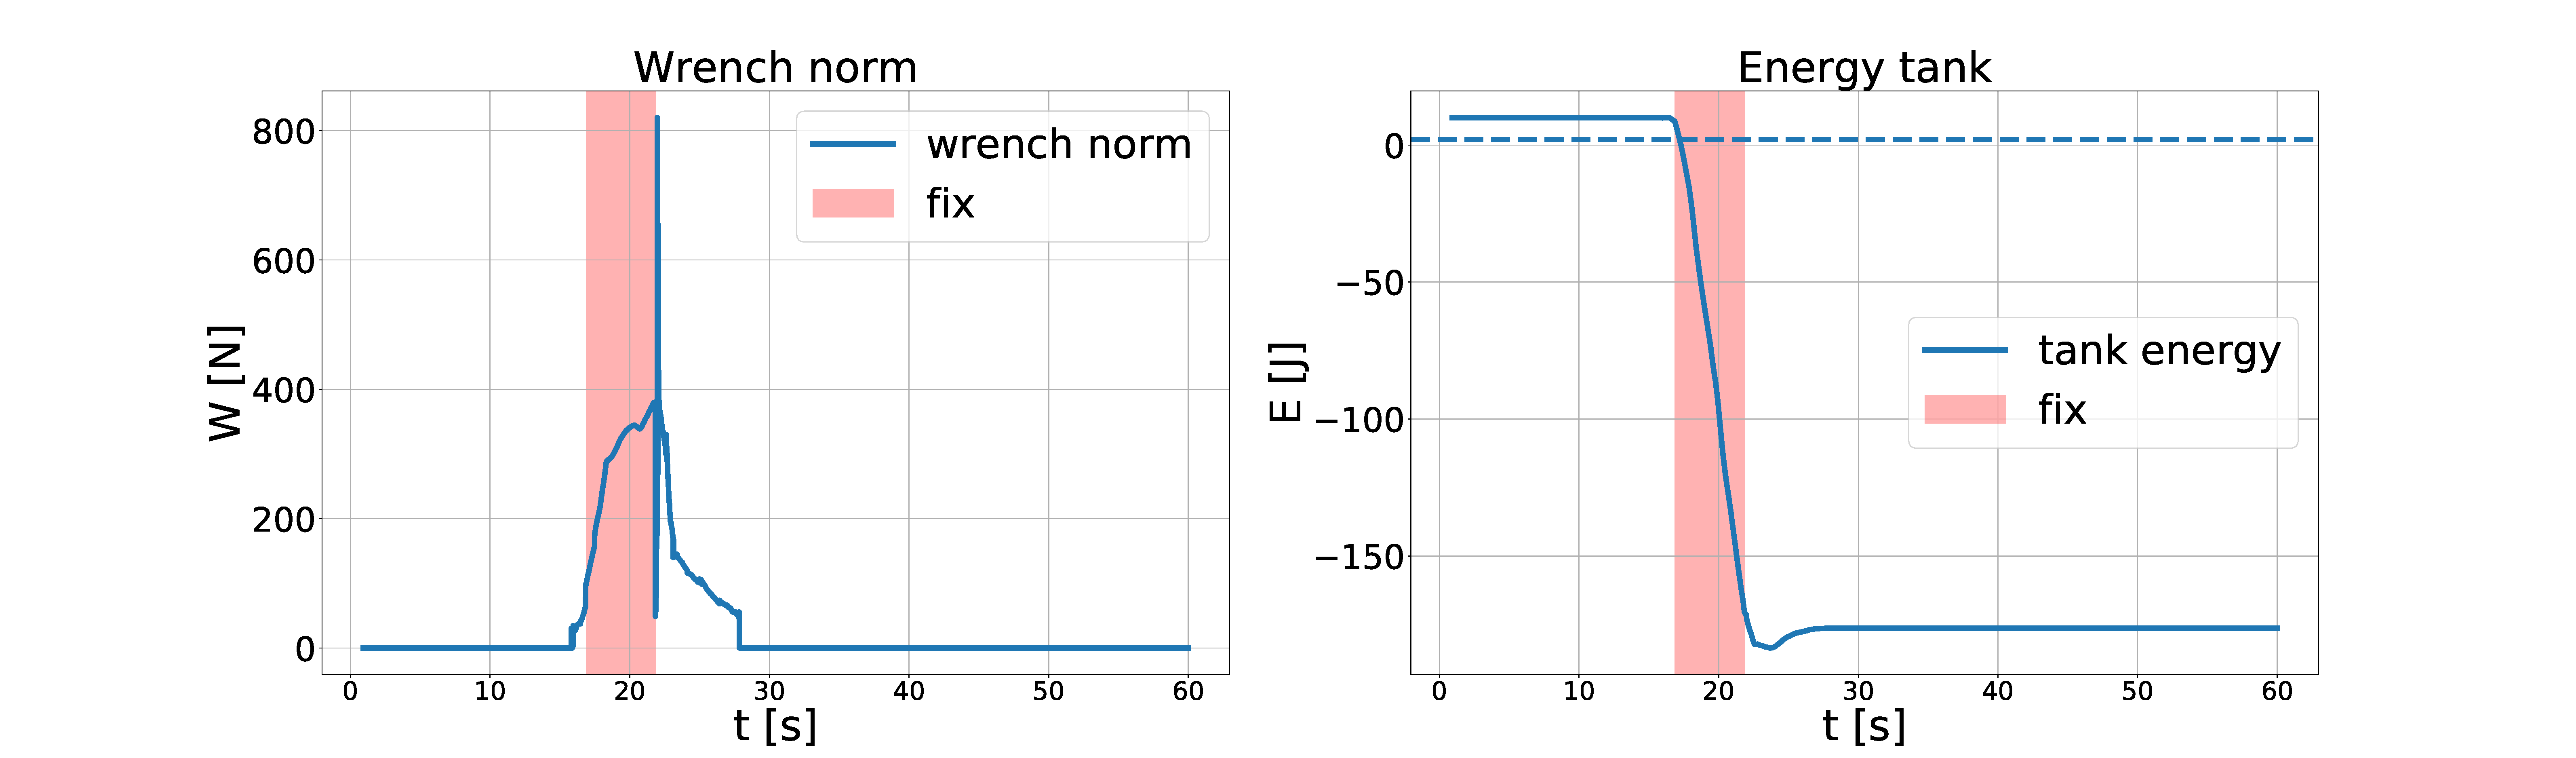
\includegraphics[width=\linewidth]{figures/fix_experiment/wrench_tank_without_tank.pdf}
    \caption{without tank}
\end{subfigure}
\hspace*{-1.35cm} 
\begin{subfigure}{1.3\columnwidth}
    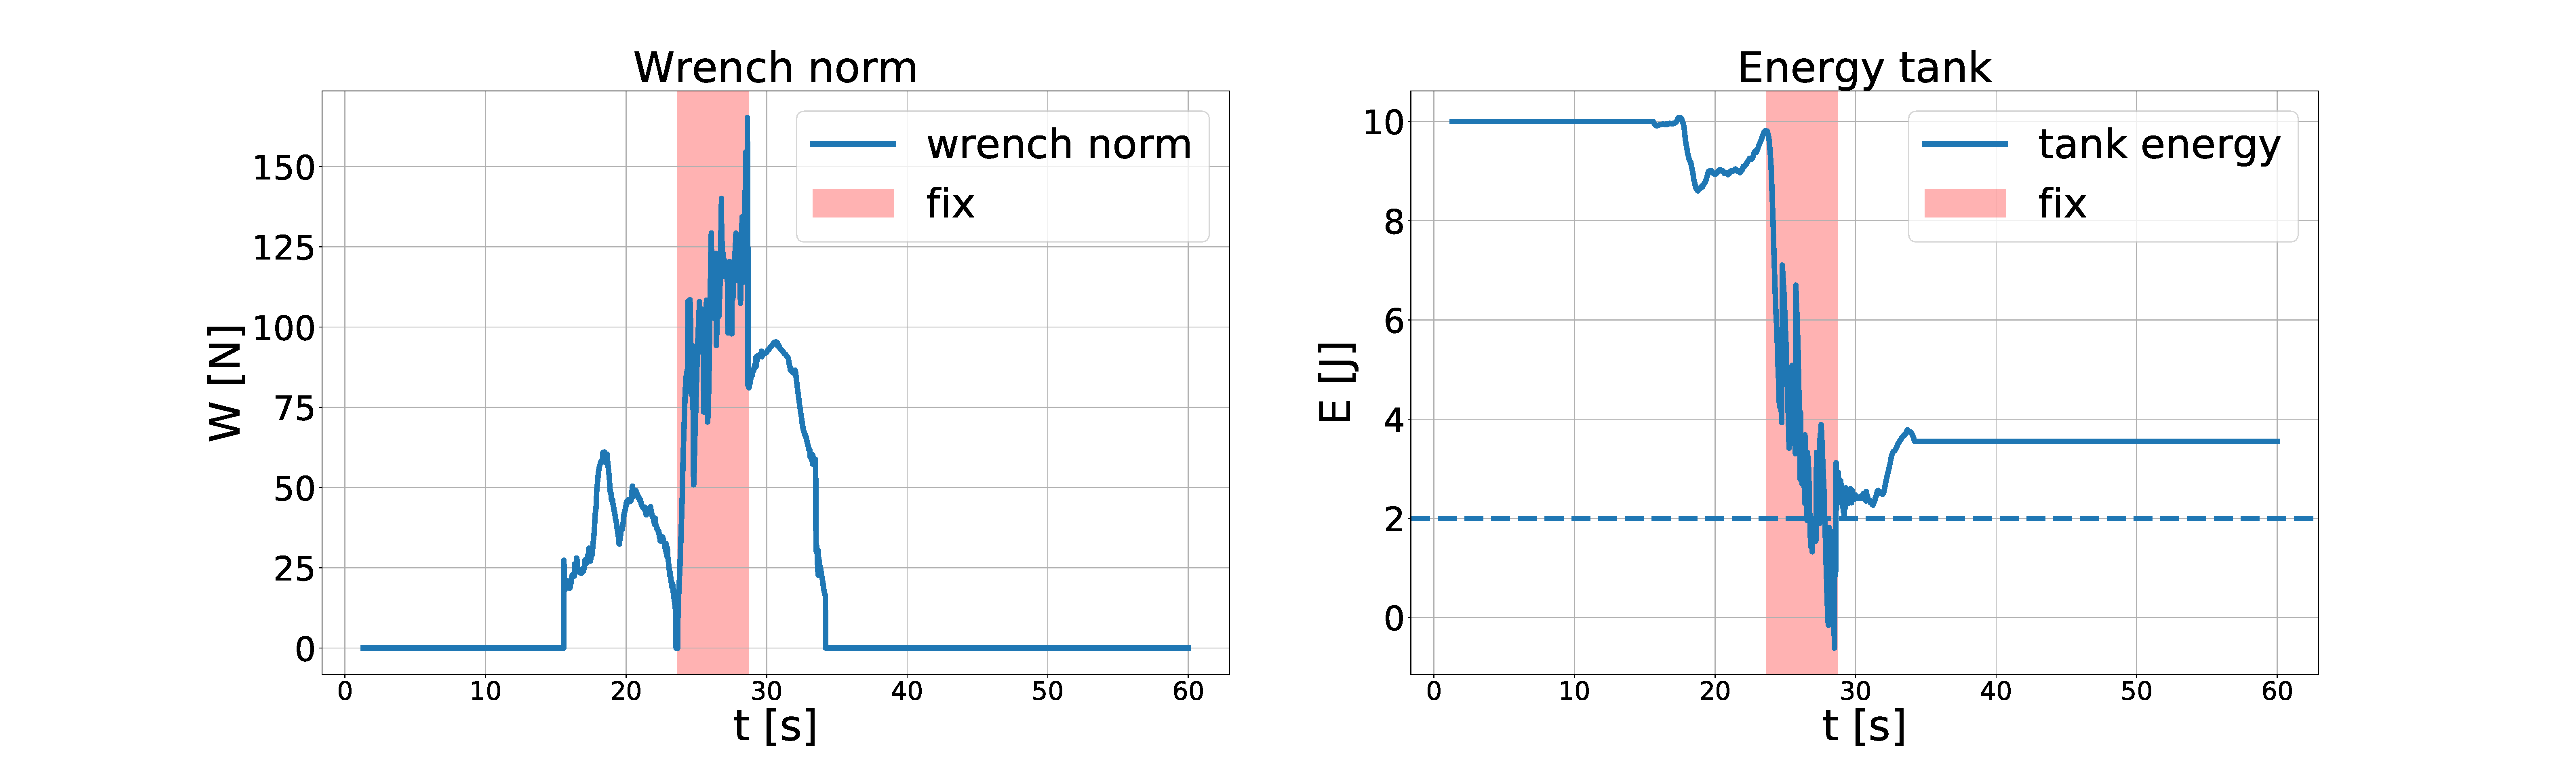
\includegraphics[width=\linewidth]{figures/fix_experiment/wrench_tank_with_tank.pdf}
    \caption{with tank}
\end{subfigure}
\hfill
\caption{The figure shows the interaction wrench and energy left in the tank during the task execution. The shaded area is the interval of time where the articulated object is fixed.  }\label{fig:methods_comparison}
\end{figure}
\subsection{Real world experiments}
Our RoyalPanda test platform consists of a holonomic mobile base equipped with a 7-DOF manipulator. The robot's wrist mounts a custom set of fingers as shown in \fig\ref{fig:custom_fingers}. This hardware adaptation simplifies the problem without limiting the capabilities of the platform. We run the presented algorithm on a Intel Core i7-8550U quad-core processor (1.8 GHz, up to 4.0 GHz) and use 8 threads for parallel forward sampling of rollouts. All control parameters are summarized in \tab \add{add table of parameters}. The target velocity commands are tracked by a PI controller which converts these into motor torques. The omnidirectional base is controlled by sending velocity commands to the mecanum wheel controller. The arm's low-level controller runs at 1KHz while the base mecanum controller runs at 50Hz.


The experiment goal is to demonstrate that the algorithm can be deployed on a real platform at high control rates. For this purpose, we perform a door opening experiment. The door and the robot base are tracked via a VICON system, eliminating the need for precise state estimation. We plan to remove this limitation in future work. In order to qualitatively evaluate the algorithm's replanning capabilities, we disturb the manipulator during the opening phase releasing the contact between the handle and the finger. As we can see in the accompanying video, the controller is able to re-plan a feasible trajectory to the handle and successfully perform the task.     
In \fig\ref{fig:mobile_manipulation_hardware} the magnitudes of the base and end-effector velocities are plotted to visualize the whole-body coordination throughout the manipulation task.

\begin{figure}[t]
\centering
\begin{subfigure}{\columnwidth}
    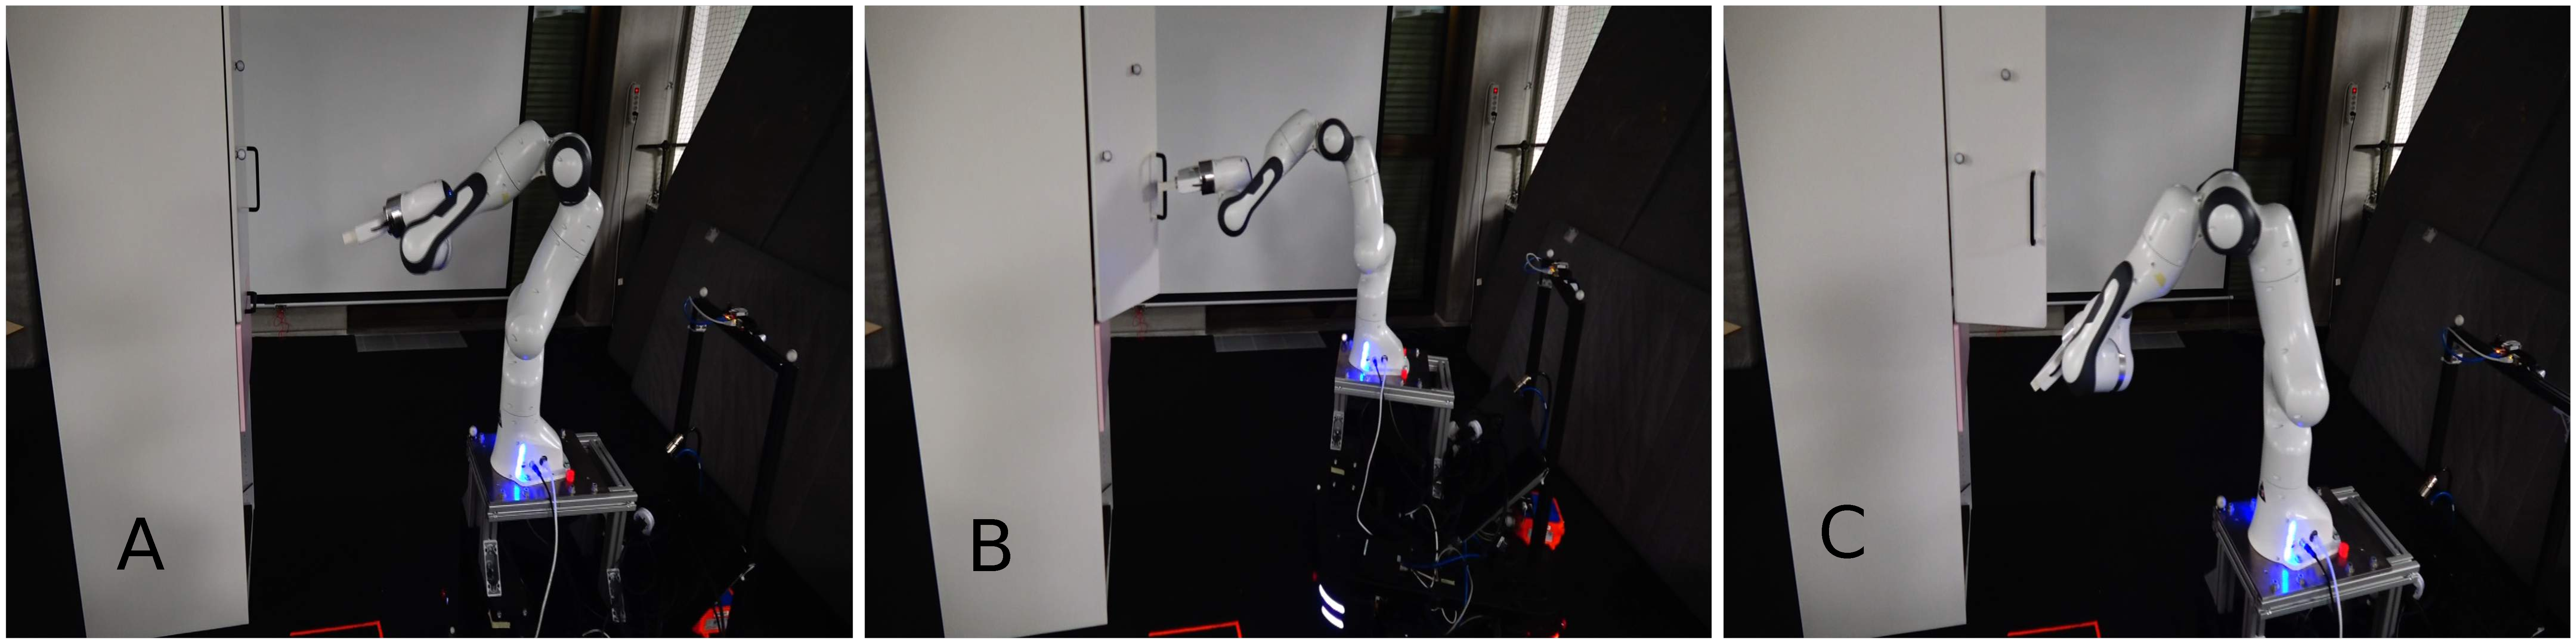
\includegraphics[width=\linewidth]{figures/mobile_robot_montage-compressed.pdf}
    \caption{Extract of the manipulation sequence. In A the robot reaches an estimated target region near the handle. In B the door is opened. In C the end-effector moves back to the starting pose.}
\end{subfigure}%
\hfill
\begin{subfigure}{\columnwidth}
    \includegraphics[trim={0 10 0 50},clip,width=\linewidth]{figures/velocity_norm_annotated.pdf}
    \caption{Velocity contributions of the base and of the end-effector with respect to the base frame. These results show that whole-body coordination occurs at all the times of the manipulation task.}
\end{subfigure}%}
\caption{Whole-body door opening with a mobile manipulator.} \label{fig:mobile_manipulation_hardware}
\end{figure}